\documentclass{article}

\usepackage{graphicx}
\usepackage{subcaption}

% these packages let you do math
\usepackage{amsmath}
\usepackage{amssymb}

% we need these packages for fancy R tables
\usepackage{booktabs}
\usepackage{float}
\usepackage{colortbl}
\usepackage{xcolor}

% these packages play with the spacing/margins of the document. Uncomment the commands on lines 16 and 17 to see what they do.
\usepackage{a4wide}\usepackage{setspace}
\usepackage{geometry}
\usepackage{parskip}
%\doublespacing
%\geometry{margin=1.5in}

% this package helps us with including images. Setting the graphics path makes it easier to refer to things in the \includegraphics command.
\usepackage{graphicx}
\graphicspath{ {../figures/} }

% make some hyperlinks using the \href command
\usepackage{hyperref}
\hypersetup{
    colorlinks=true,
    linkcolor=black,
    urlcolor=blue
}

% set the author, title, and date of the document. \maketitle adds it to the document.
\author{Seungwoon Shin}
\title{My Paper on NLSY02 Data}
\date{Sping 2022}

\begin{document}
\maketitle

\section{Brief Analysis}
The main objective of this paper is to compare the mean number of arrests between 1997 and 2002 by race and gender. 

\begin{figure}[H]

    \caption{Mean Number of Arrests by Race and Gender}
    \centering
    \begin{subfigure}[b]{0.49\textwidth}
        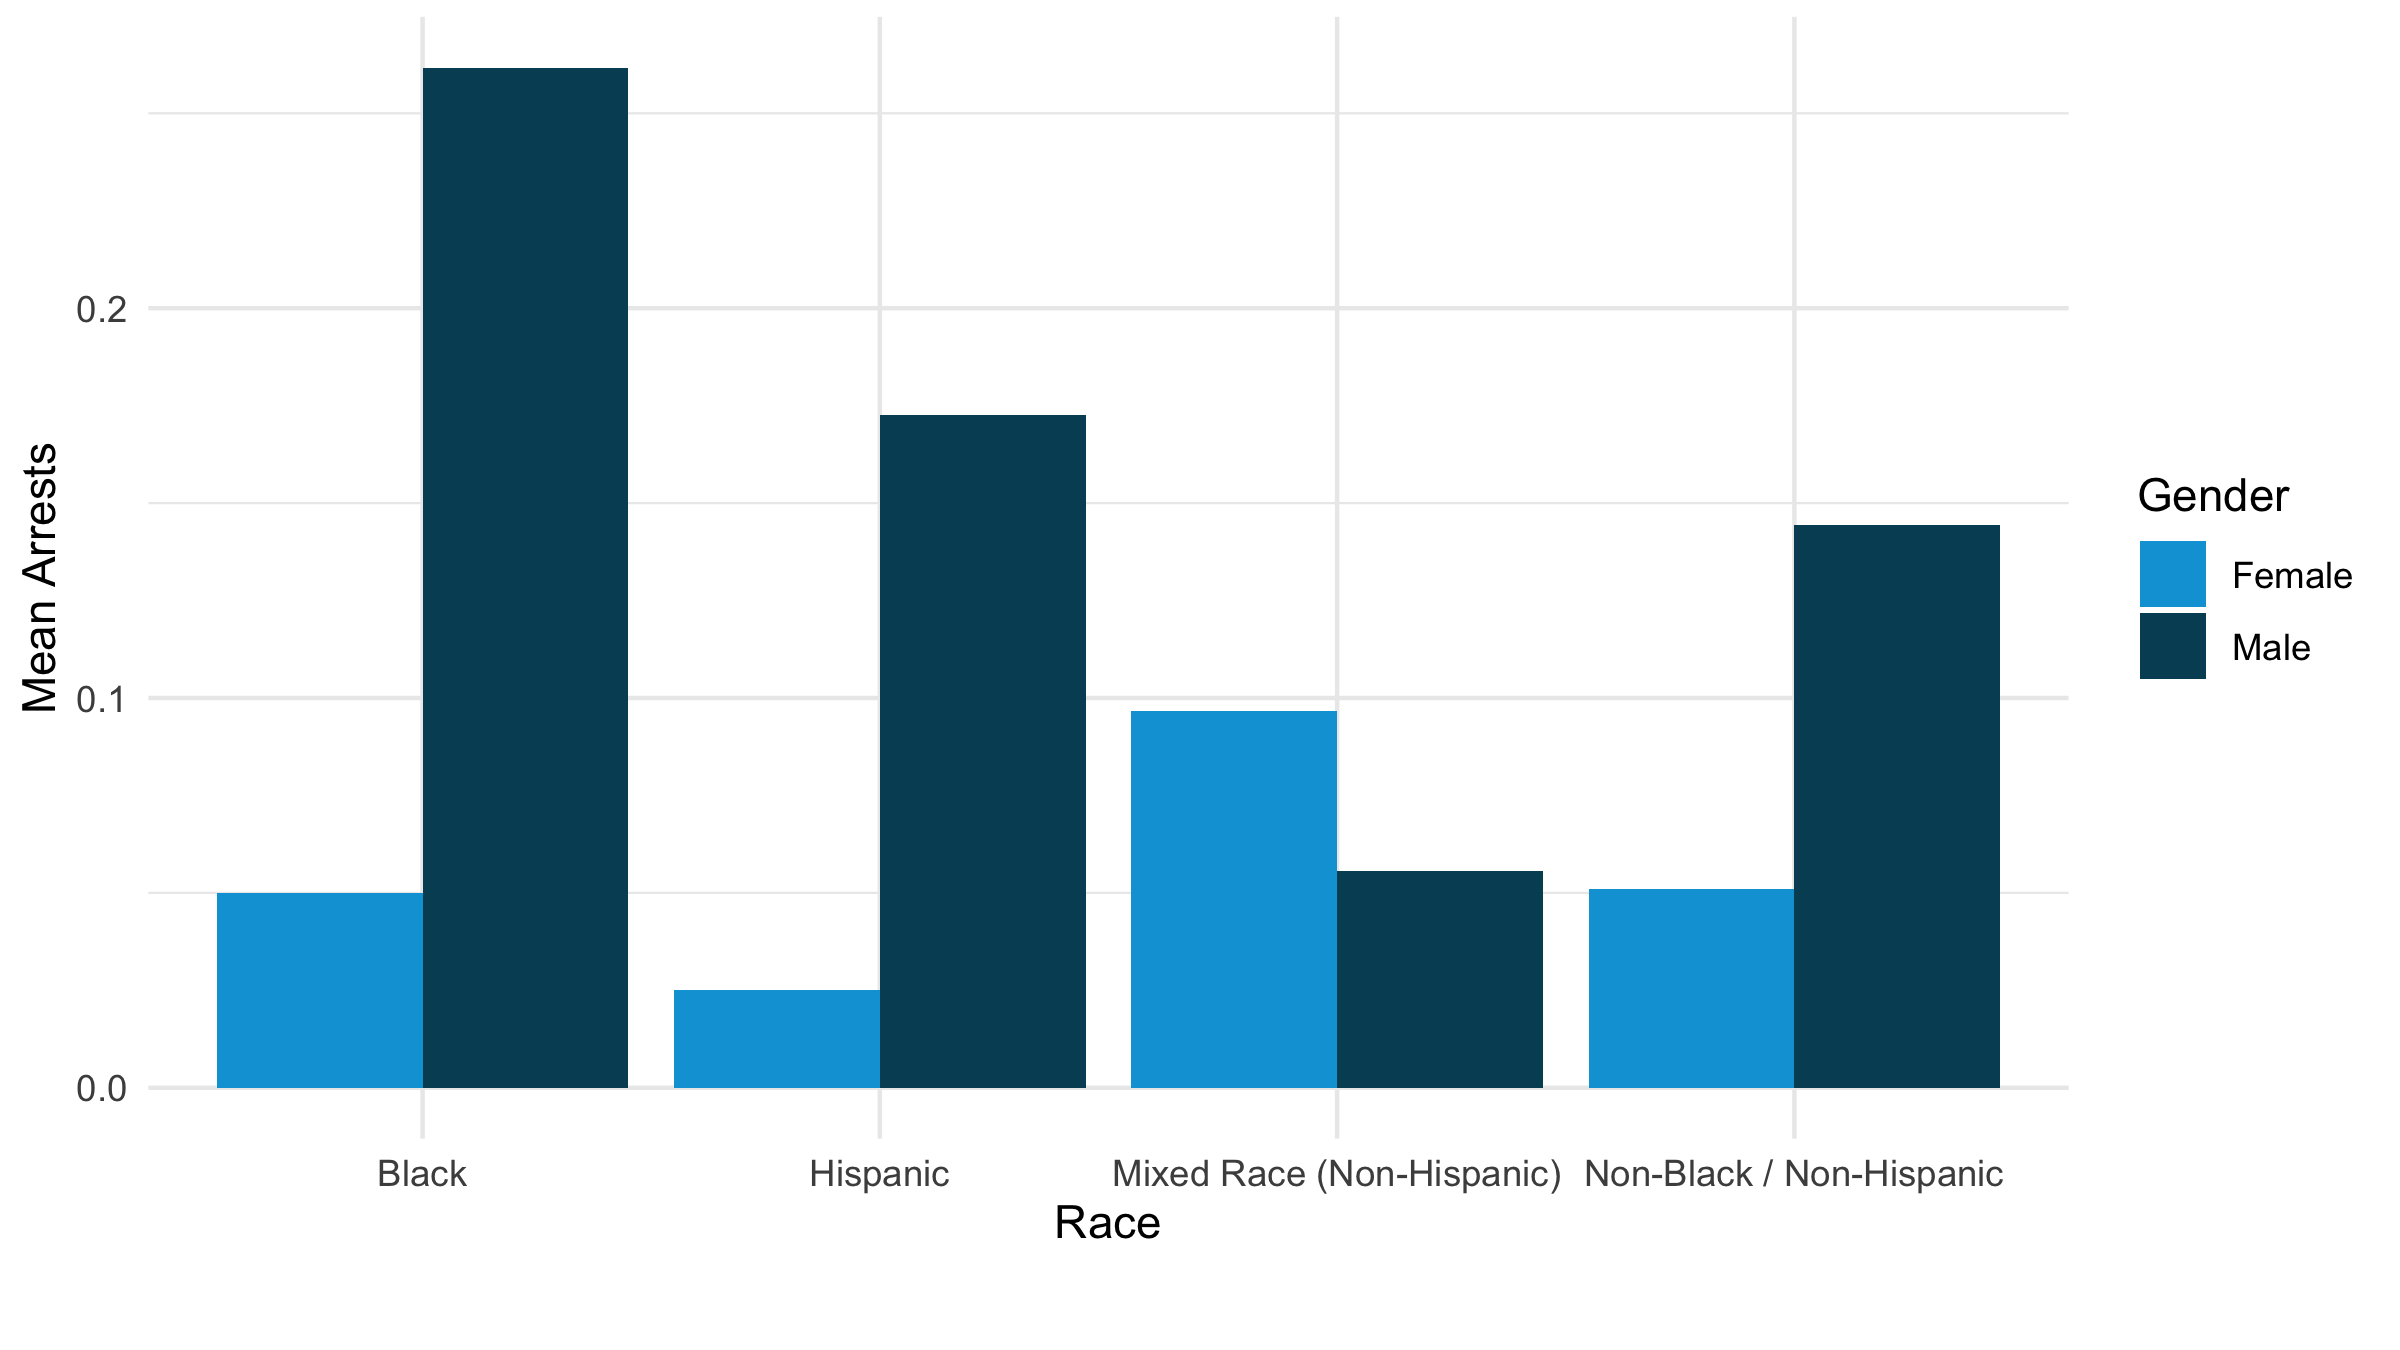
\includegraphics[width=\textwidth]{arrests_by_racegender}
        \caption{1997}
    \end{subfigure}
    \begin{subfigure}[b]{0.49\textwidth}
        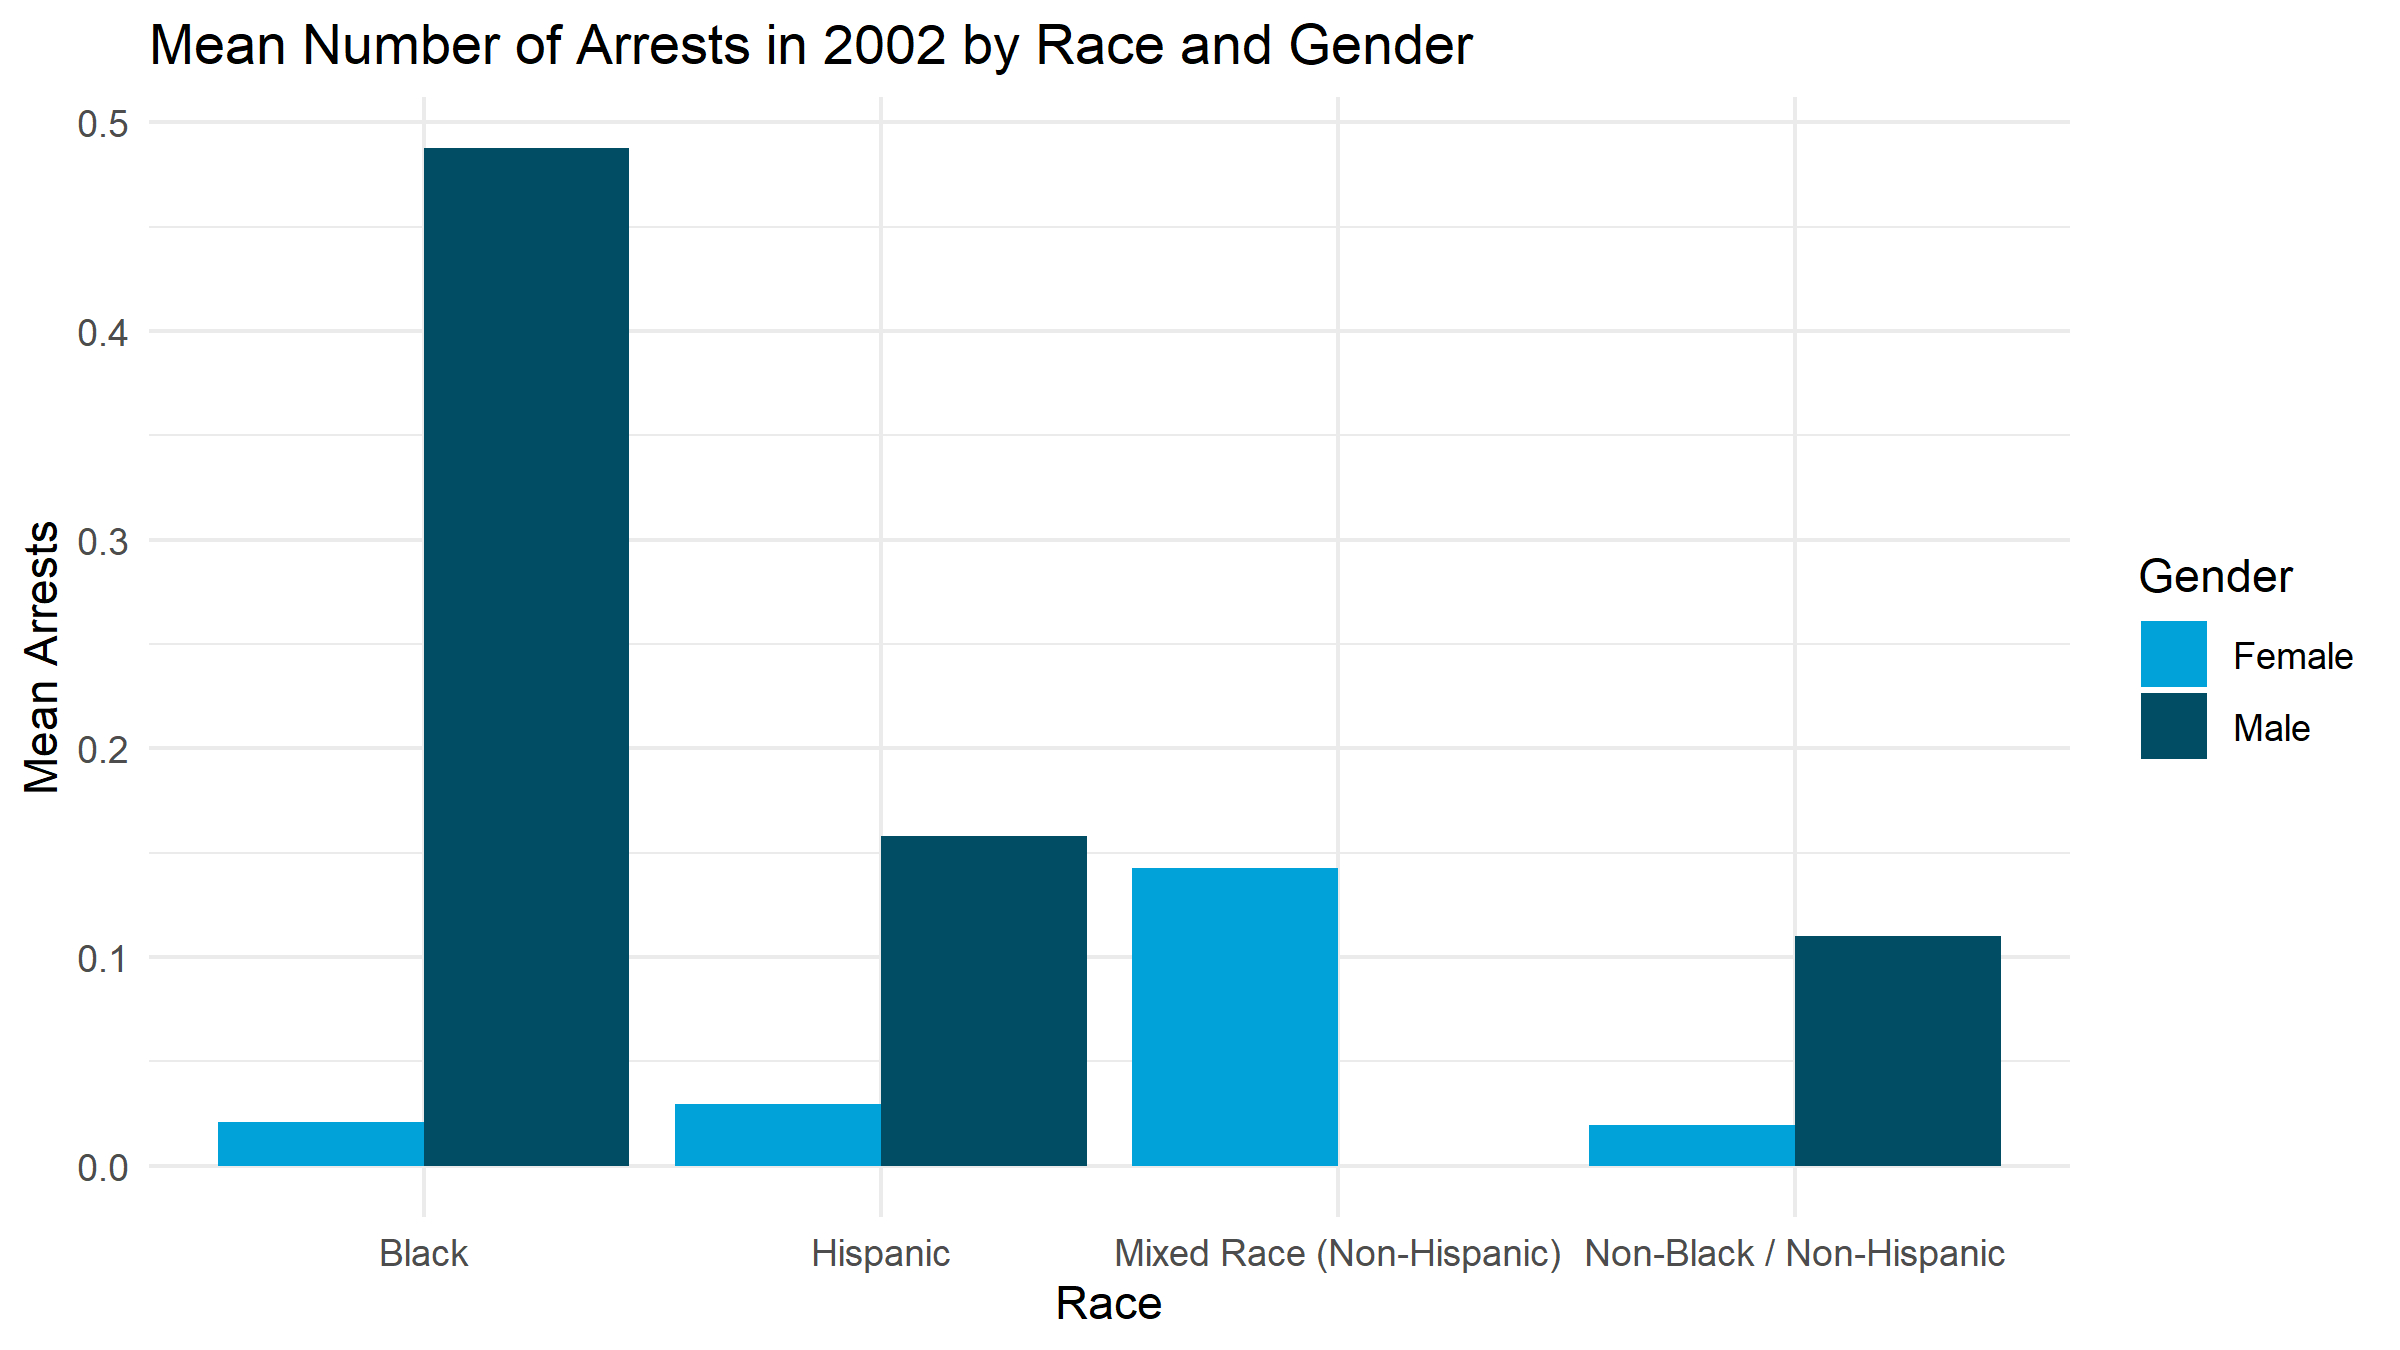
\includegraphics[width=\textwidth]{02arrests_by_racegender}
        \caption{2002}
    \end{subfigure}
    \label{fig:graph}


\end{figure}

\begin{table}[H]

\caption{\label{tab:tab:summarystats}Mean arrests in 1997 by Race and Gender}
\centering
\begin{tabular}[t]{lrrrr}
\toprule
Gender & Black & Hispanic & Mixed Race Non Hispanic & Non Black Non Hispanic\\
\midrule
\cellcolor{gray!6}{Female} & \cellcolor{gray!6}{0.0500481} & \cellcolor{gray!6}{0.0251497} & \cellcolor{gray!6}{0.0967742} & \cellcolor{gray!6}{0.0510659}\\
Male & 0.2617230 & 0.1725441 & 0.0555556 & 0.1443401\\
\bottomrule
\end{tabular}
\end{table}

\begin{table}[H]

\caption{\label{tab:tab:summarystats}Mean arrests in 2002 by Race and Gender}
\centering
\begin{tabular}[t]{lrrrr}
\toprule
Gender & Black & Hispanic & Mixed Race Non Hispanic & Non Black Non Hispanic\\
\midrule
\cellcolor{gray!6}{Female} & \cellcolor{gray!6}{0.0211268} & \cellcolor{gray!6}{0.0298013} & \cellcolor{gray!6}{0.1428571} & \cellcolor{gray!6}{0.0193192}\\
Male & 0.4876712 & 0.1579509 & 0.0000000 & 0.1099476\\
\bottomrule
\end{tabular}
\end{table}

As we have seen Figure \ref{fig:graph} and the Tables, the male is more likely to commit crimes than the female regardless of race and year except for mixed-race(non-Hispanic). The largest mean number of arrests is from Black male regardless of years. The mean number of arrests increased over time for Black males whereas it decreased for the rest of the other males. The mean number of arrests has increased for females regardless of the race except for Blacks.
\section{Regression}




% Table created by stargazer v.5.2.3 by Marek Hlavac, Social Policy Institute. E-mail: marek.hlavac at gmail.com
% Date and time: Wed, Apr 27, 2022 - 1:18:29 AM
\begin{table}[!htbp] \centering 
  \caption{Regression Output. Omitted category is Black Females.} 
  \label{tab:regression} 
\begin{tabular}{@{\extracolsep{5pt}}lc} 
\\[-1.8ex]\hline 
\hline \\[-1.8ex] 
 & \multicolumn{1}{c}{\textit{Dependent variable:}} \\ 
\cline{2-2} 
\\[-1.8ex] & Arrests in 1997 \\ 
\hline \\[-1.8ex] 
 Hispanic & $-$0.055$^{***}$ \\ 
  & (0.019) \\ 
  & \\ 
 Mixed Race (Non-Hispanic) & $-$0.084$^{*}$ \\ 
  & (0.043) \\ 
  & \\ 
 Non-Black / Non-Hispanic & $-$0.056$^{***}$ \\ 
  & (0.017) \\ 
  & \\ 
 Male & 0.134$^{***}$ \\ 
  & (0.012) \\ 
  & \\ 
 Constant & 0.087$^{***}$ \\ 
  & (0.013) \\ 
  & \\ 
\hline \\[-1.8ex] 
Observations & 7,692 \\ 
R$^{2}$ & 0.018 \\ 
Adjusted R$^{2}$ & 0.017 \\ 
Residual Std. Error & 0.526 (df = 7687) \\ 
F Statistic & 34.624$^{***}$ (df = 4; 7687) \\ 
\hline 
\hline \\[-1.8ex] 
\textit{Note:}  & \multicolumn{1}{r}{$^{*}$p$<$0.1; $^{**}$p$<$0.05; $^{***}$p$<$0.01} \\ 
\end{tabular} 
\end{table} 


The sign of dependent variables indicates that Male with a positive coefficient is likely to commit crimes. Namely, it leads an increase in the mean number of arrests in 1997. In contrast, the rest induces a decrease in the mean number of arrests. The dependent variable 'Male' also partially implies the largest mean number of arrests from Blacks.

\newpage

% Table created by stargazer v.5.2.3 by Marek Hlavac, Social Policy Institute. E-mail: marek.hlavac at gmail.com
% Date and time: Wed, Apr 27, 2022 - 1:17:34 AM
\begin{table}[!htbp] \centering 
  \caption{Regression Output. Omitted category is Black Females.} 
  \label{tab:regression} 
\begin{tabular}{@{\extracolsep{5pt}}lc} 
\\[-1.8ex]\hline 
\hline \\[-1.8ex] 
 & \multicolumn{1}{c}{\textit{Dependent variable:}} \\ 
\cline{2-2} 
\\[-1.8ex] & Arrests in 2002 \\ 
\hline \\[-1.8ex] 
 Hispanic & $-$0.159$^{***}$ \\ 
  & (0.038) \\ 
  & \\ 
 Mixed Race (Non-Hispanic) & $-$0.174$^{**}$ \\ 
  & (0.083) \\ 
  & \\ 
 Non-Black / Non-Hispanic & $-$0.189$^{***}$ \\ 
  & (0.035) \\ 
  & \\ 
 Male & 0.194$^{***}$ \\ 
  & (0.022) \\ 
  & \\ 
 Constant & 0.155$^{***}$ \\ 
  & (0.026) \\ 
  & \\ 
\hline \\[-1.8ex] 
Observations & 8,621 \\ 
R$^{2}$ & 0.015 \\ 
Adjusted R$^{2}$ & 0.014 \\ 
Residual Std. Error & 1.019 (df = 8616) \\ 
F Statistic & 32.033$^{***}$ (df = 4; 8616) \\ 
\hline 
\hline \\[-1.8ex] 
\textit{Note:}  & \multicolumn{1}{r}{$^{*}$p$<$0.1; $^{**}$p$<$0.05; $^{***}$p$<$0.01} \\ 
\end{tabular} 
\end{table} 


Unlike previous Table 3, the absolute value of all dependent variable coefficients has increased. This indicates that some of the categories such as Black male remarkably increased in the mean number of arrests in 2002 while the other categories such as Mixed race (non-Hispanic) male decreased a lot. 

\end{document}
